\begin{apendicesenv}

\partapendices
\chapter{Tabelas de Requisitos}

\begin{table}[h]
    \centering
    \caption{Comparação de funcionalidades entre Hotmart e Udemy - Parte 1}
    \label{tab:comparacao_hotmart_udemy}
    \begin{adjustbox}{width=\textwidth}
    \begin{tabular}{|p{5cm}|p{5cm}|p{5cm}|}
        \hline
        \textbf{Critério} & \textbf{Hotmart} & \textbf{Udemy} \\
        \hline
        \textbf{Criação de cursos} & Permite a criação e hospedagem de cursos online. & Oferece ferramentas para criação e publicação de cursos. \\
        \hline
        \textbf{Área do usuário} & Gestão dos dados do usuário, meios de pagamento, preferências do sistema. & Gestão dos dados do usuário, meios de pagamento, preferências do sistema, gestão de API para clientes. \\
        \hline
        \textbf{Categorização} & Categorização de cursos em dois níveis. & Categorização de cursos em dois níveis. \\
        \hline
        \textbf{Lista de cursos pessoais} & Listagem de cursos que estão sendo consumidos pelo usuário. & Listagem de cursos que estão sendo consumidos pelo usuário. \\
        \hline
        \textbf{Suporte a material escrito} & Hospedagem de materiais textuais digitais. & Não tem ênfase em hospedagem de materiais escritos. \\
        \hline
        \textbf{Suporte a Vídeos} & Hospedagem de vídeos integrada. & Hospedagem de vídeos com suporte a legendas. \\
        \hline
        \textbf{Integração de Pagamentos} & Sistema de pagamento integrado (HotPay). & Sistema de pagamento próprio (Udemy Payments). \\
        \hline
        \textbf{Métodos de Monetização} & Venda direta, assinaturas, afiliados. & Venda direta, cupons de desconto, promoções. \\
        \hline
        \textbf{Afiliados} & Programa de afiliados robusto. & Programa de afiliados disponível. \\
        \hline
        \textbf{Personalização} & Personalização limitada da página de vendas. & Personalização do conteúdo do curso. \\
        \hline
        \textbf{Certificados} & Certificados customizáveis para alunos. & Certificados para conclusão de curso. \\
        \hline
        \textbf{Ferramentas de Marketing} & Ferramentas avançadas de marketing e automação. & Ferramentas básicas de marketing e promoção. \\
        \hline
        \textbf{Análise de Dados} & Relatórios detalhados de vendas e desempenho. & Análises de desempenho do curso e dos alunos. \\
        \hline
        \textbf{Comunidade} & Comunidade de produtores e afiliados. & Comunidade de instrutores e alunos. \\
        \hline
        \textbf{Suporte ao Instrutor} & Suporte por e-mail e chat. & Suporte por e-mail e centro de ajuda. \\
        \hline
        \textbf{Aplicativo Móvel} & Aplicativo para alunos e produtores. & Aplicativo móvel para alunos. \\
        \hline
    \end{tabular}
    \end{adjustbox}

    \vspace{5mm}
    {\footnotesize Fonte: Autores} 

\end{table}

\begin{table}[h]
    \centering
    \caption{Comparação de funcionalidades entre Hotmart e Udemy - Parte 2}
    \label{tab:comparacao_hotmart_udemy2}
    \begin{adjustbox}{width=\textwidth}
    \begin{tabular}{|p{5cm}|p{5cm}|p{5cm}|}
\hline
\textbf{Integrações} & Injtegração com ferramentas de e-mail e CRM (ferramenta de gestão de relacionamento com clientes). & Integração com ferramentas de terceiros via API. \\
\hline
\textbf{Segurança} & Proteção contra pirataria e fraudes. & Proteção básica contra pirataria. \\
\hline
\textbf{Gamificação} & Recursos limitados de gamificação. & Recursos de gamificação (badges, quizzes). \\
\hline
\textbf{Acessibilidade} & Recursos básicos de acessibilidade. & Legendas e transcrições para vídeos. \\
\hline
\textbf{Preços} & Taxas sobre vendas e planos de assinatura. & Taxas sobre vendas e compartilhamento de receita. \\
\hline
\end{tabular}
\end{adjustbox}

\vspace{5mm}
{\footnotesize Fonte: Autores} 

\end{table}


\begin{table}[h]
    \centering
    \caption{Priorização de Requesitos utilizando MoSCoW - Must Have}
    \label{tab:priorizacao_moscow}
    \begin{adjustbox}{width=\textwidth}
        \begin{tabular}{|p{2.5cm}|p{5cm}|p{5cm}|p{4cm}|}
        \hline
        \textbf{Requisito} & \textbf{Critério} & \textbf{Prioridade} & \textbf{Motivação} \\
        \hline
        RF01 & Criação de cursos & Must Have & Recurso essencial, pois sem ele a plataforma não cumpre seu propósito de oferecer cursos online. \\
        \hline
        RF02 & Área do usuário & Must Have & Fundamental para que os alunos e instrutores possam gerenciar seus cursos, progresso e configurações. \\
        \hline
        RF03 & Categorização & Must Have & Permite que os cursos sejam organizados por temas, facilitando a navegação e descoberta de conteúdos relevantes. \\
        \hline
        RF04 & Lista de cursos pessoais & Must Have & Possibilita que os alunos acompanhem seu progresso e retomem cursos facilmente, melhorando a experiência de aprendizado. \\
        \hline
        RF05 & Suporte a material escrito & Must Have & Muitos materiais se adaptam melhor em formato de texto como artigos e apostilas. \\
        \hline
        RF06 & Suporte a vídeos & Must Have & A principal forma de ensino em plataformas digitais é por meio de vídeos, tornando essa funcionalidade indispensável. \\
        \hline
        RF07 & Suporte ao instrutor & Must Have & Necessário para garantir que criadores de cursos recebam suporte técnico. \\
        \hline
        RF08 & Segurança & Must Have & Protege conteúdos contra fraudes, garantindo a confiabilidade da plataforma. \\
        \hline
    \end{tabular}
\end{adjustbox}

\vspace{5mm}
{\footnotesize Fonte: Autores} 
\end{table}


\begin{table}[h]
    \centering
    \caption{Priorização de Requesitos utilizando MoSCoW - Should Have}
    \label{tab:priorizacao_moscow2}
    \begin{adjustbox}{width=\textwidth}
        \begin{tabular}{|p{2.5cm}|p{5cm}|p{5cm}|p{4cm}|}
            \hline
            \textbf{Requisito} & \textbf{Critério} & \textbf{Prioridade} & \textbf{Motivação} \\
            \hline
            RF09 & Integração de pagamentos & Should Have & Funcionalidade importante para o funcionamento de cursos pagos. \\
            \hline
            RF10 & Métodos de monetização & Should Have & Integração com novas ferramentas descentralizadas de pagamento como criptomoedas. \\
            \hline
            RF11 & Acessibilidade & Should Have & Importante para garantir inclusão, permitindo que pessoas com deficiência utilizem a plataforma sem barreiras. \\
            \hline
            RF12 & Preços & Should Have & Permite que os criadores definam diferentes modelos de precificação, garantindo maior flexibilidade ao criador do material. \\
            \hline
        \end{tabular}
    \end{adjustbox}
    \vspace{5mm}
    {\footnotesize Fonte: Autores} 
\end{table}


\begin{table}[h]
    \centering
    \caption{Priorização de Requisitos utilizando MoSCoW - Could Have}
    \label{tab:priorizacao_moscow3}
    \begin{adjustbox}{width=\textwidth}
        \begin{tabular}{|p{2.5cm}|p{5cm}|p{5cm}|p{4cm}|}
            \hline
            \textbf{Requisito} & \textbf{Critério} & \textbf{Prioridade} & \textbf{Motivação} \\
            \hline
            RF13 & Personalização & Could Have & A possibilidade de personalizar a interface pode melhorar a experiência do usuário, mas não afeta o funcionamento principal. \\
            \hline
            RF14 & Ferramentas de marketing & Could Have & Facilitam a divulgação da plataforma, mas está fora do escopo almejado para o projeto. \\
            \hline
            RF15 & Análise de dados & Could Have & Facilita os instrutores da plataforma, mas está fora do escopo almejado para o projeto. \\
            \hline
            RF16 & Comunidade & Could Have & Permite interações entre alunos e instrutores, aumentando o engajamento. \\
            \hline
            RF17 & Aplicativo móvel & Could Have & Facilita o acesso a cursos em dispositivos móveis, mas a versão web atende inicialmente essa demanda. \\
            \hline
            RF18 & Integrações & Could Have & Conectar com outras ferramentas pode ser útil, mas não é um requisito essencial na fase inicial. \\
            \hline
            RF19 & Gamificação & Could Have & Elementos de gamificação tornam a experiência mais atrativa para os alunos, mas não são obrigatórios para o funcionamento básico. \\
            \hline
        \end{tabular}
    \end{adjustbox}
    \vspace{5mm}
    {\footnotesize Fonte: Autores} 
\end{table}


\begin{table}[h]
    \centering
    \caption{Priorização de Requisitos utilizando MoSCoW - Won’t Have}
    \label{tab:priorizacao_moscow4}
    \begin{adjustbox}{width=\textwidth}
        \begin{tabular}{|p{2.5cm}|p{5cm}|p{5cm}|p{4cm}|}
            \hline
            \textbf{Requisito} & \textbf{Critério} & \textbf{Prioridade} & \textbf{Motivação} \\
            \hline
            RF20 & Afiliados & Won’t Have & Embora ajude na divulgação dos cursos, não é essencial no lançamento da plataforma e pode ser implementado futuramente. \\
            \hline
            RF21 & Certificados & Won’t Have & Certificados não são essenciais para o funcionamento do produto, embora agreguem para a plataforma. \\
            \hline
        \end{tabular}
    \end{adjustbox}

    \vspace{5mm}
    {\footnotesize Fonte: Autores} 
\end{table}


\chapter{Protótipo Desenvolvido}

    \begin{figure}[h]
        \centering
        \caption{Guia de estilo}
        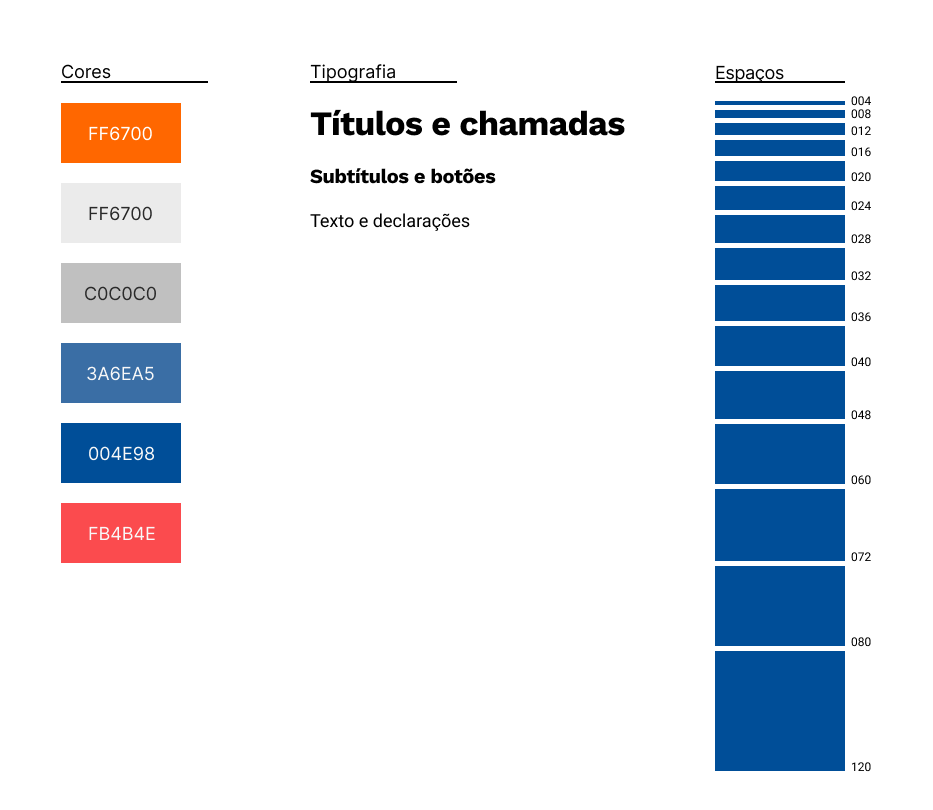
\includegraphics[width=0.8\textwidth]{figuras/guia-de-estilo.png}
        \begin{center}
            {\footnotesize Fonte: Autores}
        \end{center}
        \label{fig:guia-de-estilo}
    \end{figure}

    \begin{figure}[h]
        \centering
        \caption{Registro}
        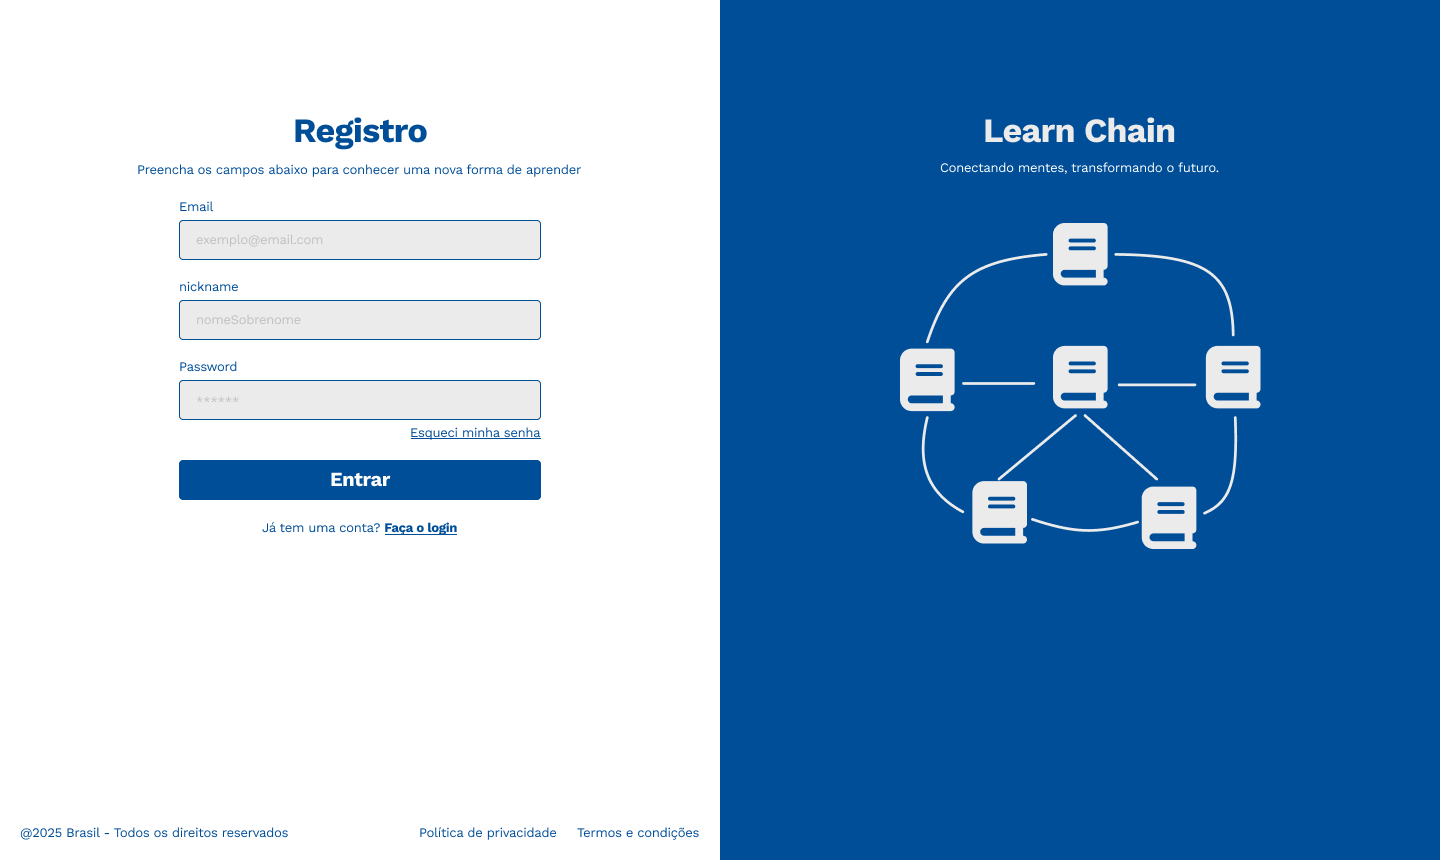
\includegraphics[width=0.8\textwidth]{figuras/Registro.png}
        \begin{center}
            {\footnotesize Fonte: Autores}
        \end{center}
        \label{fig:Registro}
    \end{figure}

    \begin{figure}[h]
        \centering
        \caption{Página inicial}
        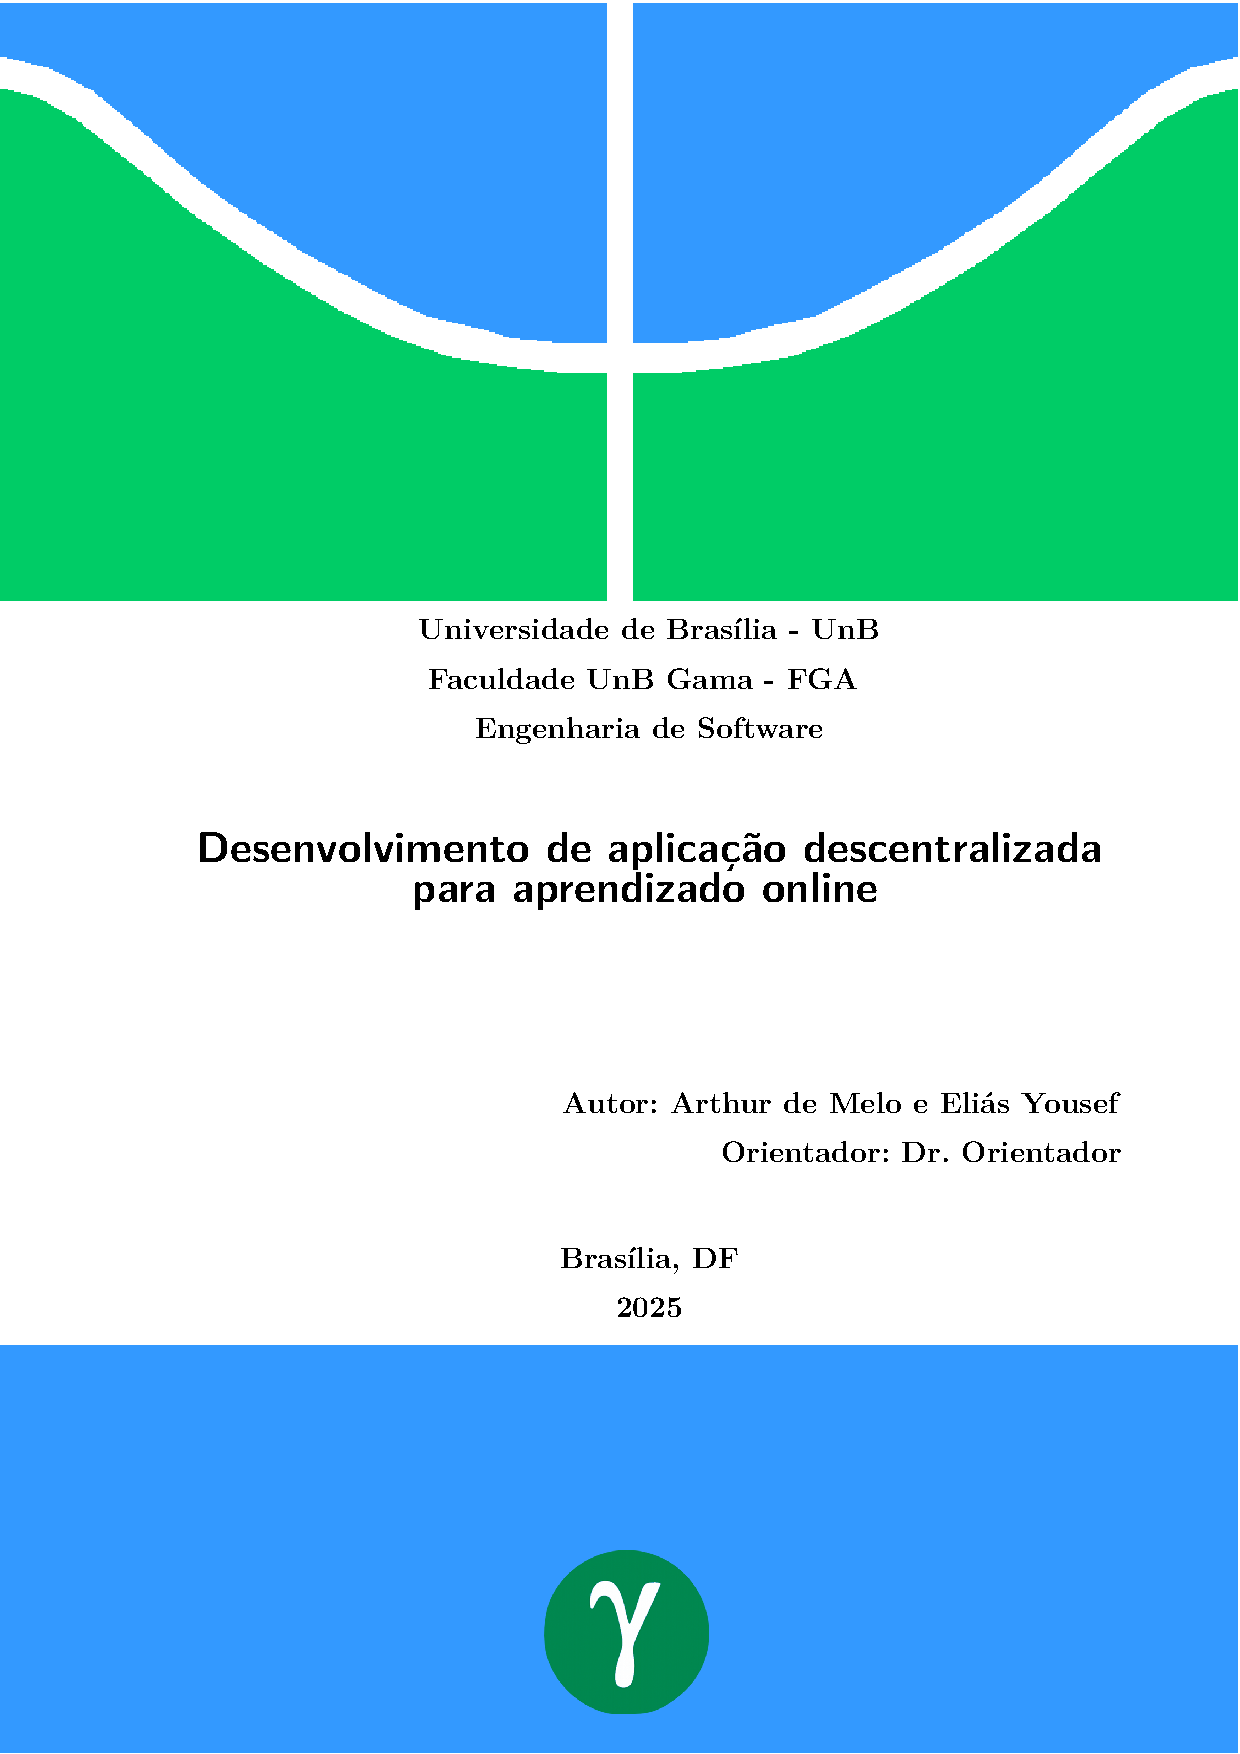
\includegraphics[width=0.8\textwidth]{figuras/main.png}
        \begin{center}
            {\footnotesize Fonte: Autores}
        \end{center}
        \label{fig:main}
    \end{figure}

    \begin{figure}[h]
        \centering
        \caption{Detalhamento do curso}
        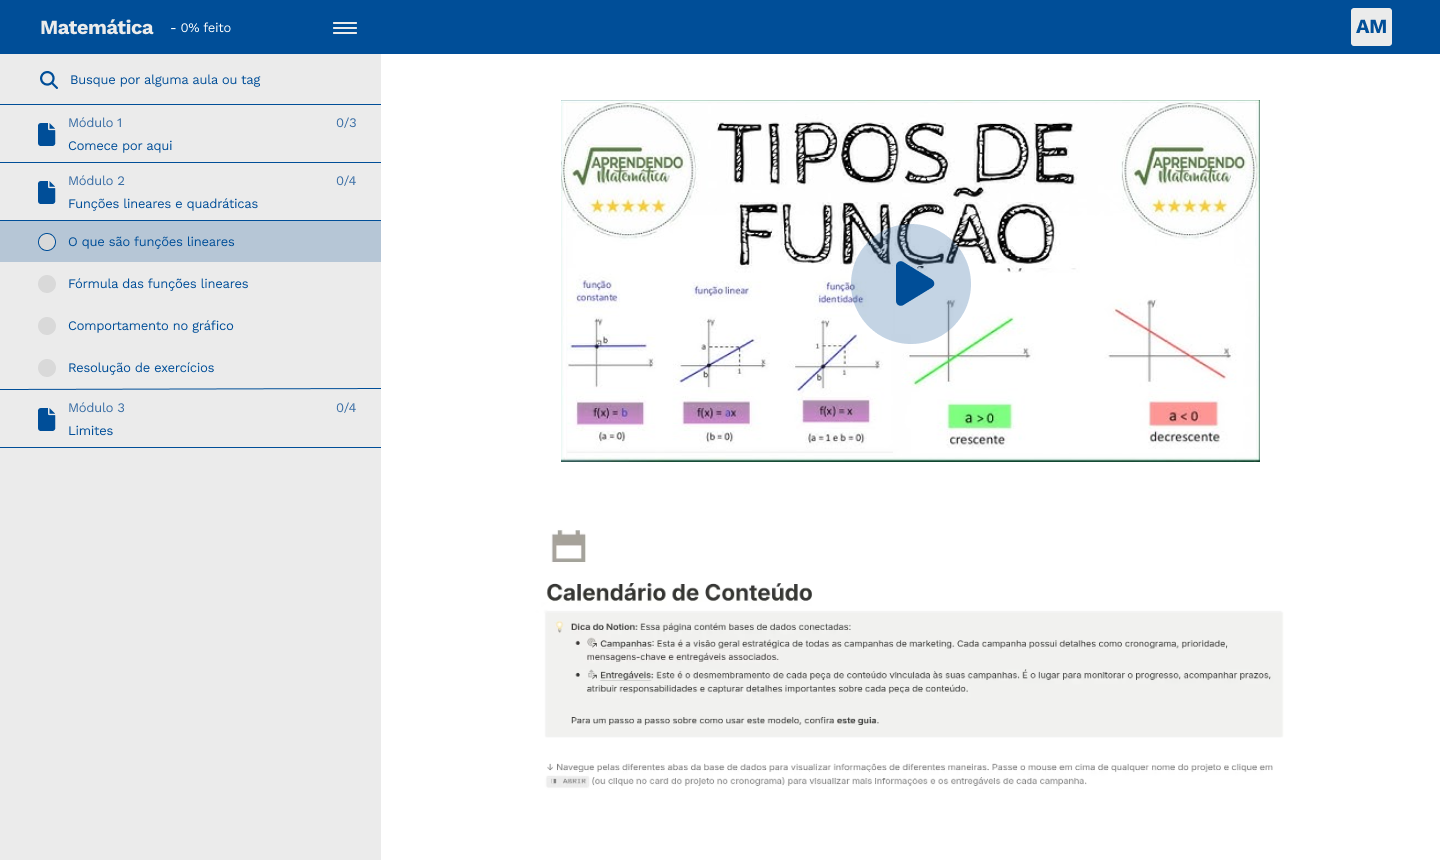
\includegraphics[width=0.8\textwidth]{figuras/detalhamento_do_curso.png}
        \begin{center}
            {\footnotesize Fonte: Autores}
        \end{center}
        \label{fig:detalhamento_do_curso}
    \end{figure}

    \begin{figure}[h]
        \centering
        \caption{Criação de conteúdo didático}
        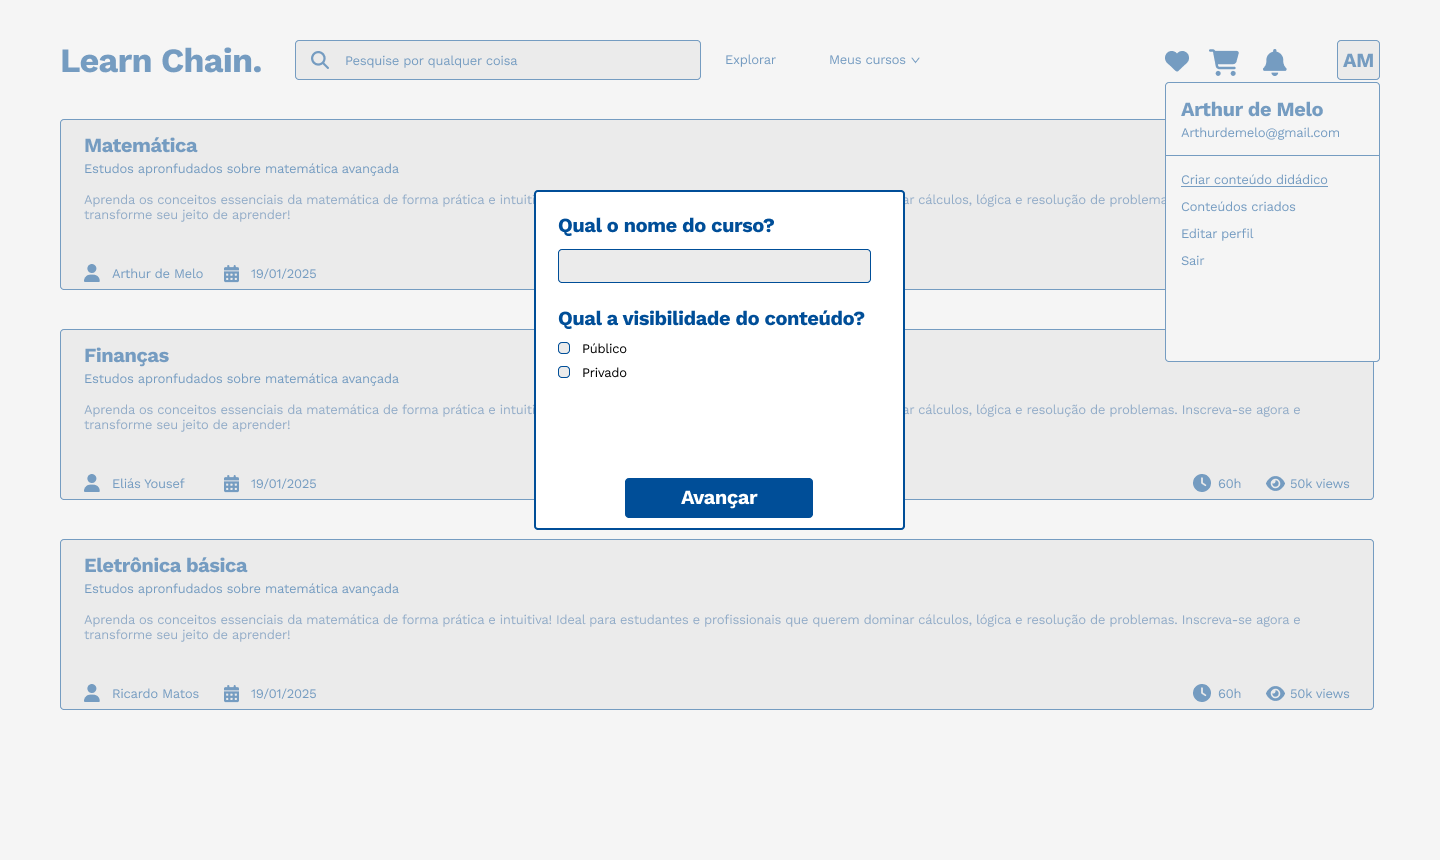
\includegraphics[width=0.8\textwidth]{figuras/Criar_conteudo_didatico.png}
        \begin{center}
            {\footnotesize Fonte: Autores}
        \end{center}
        \label{fig:Criar_conteudo_didatico}
    \end{figure}

    \begin{figure}[h]
        \centering
        \caption{Meus cursos}
        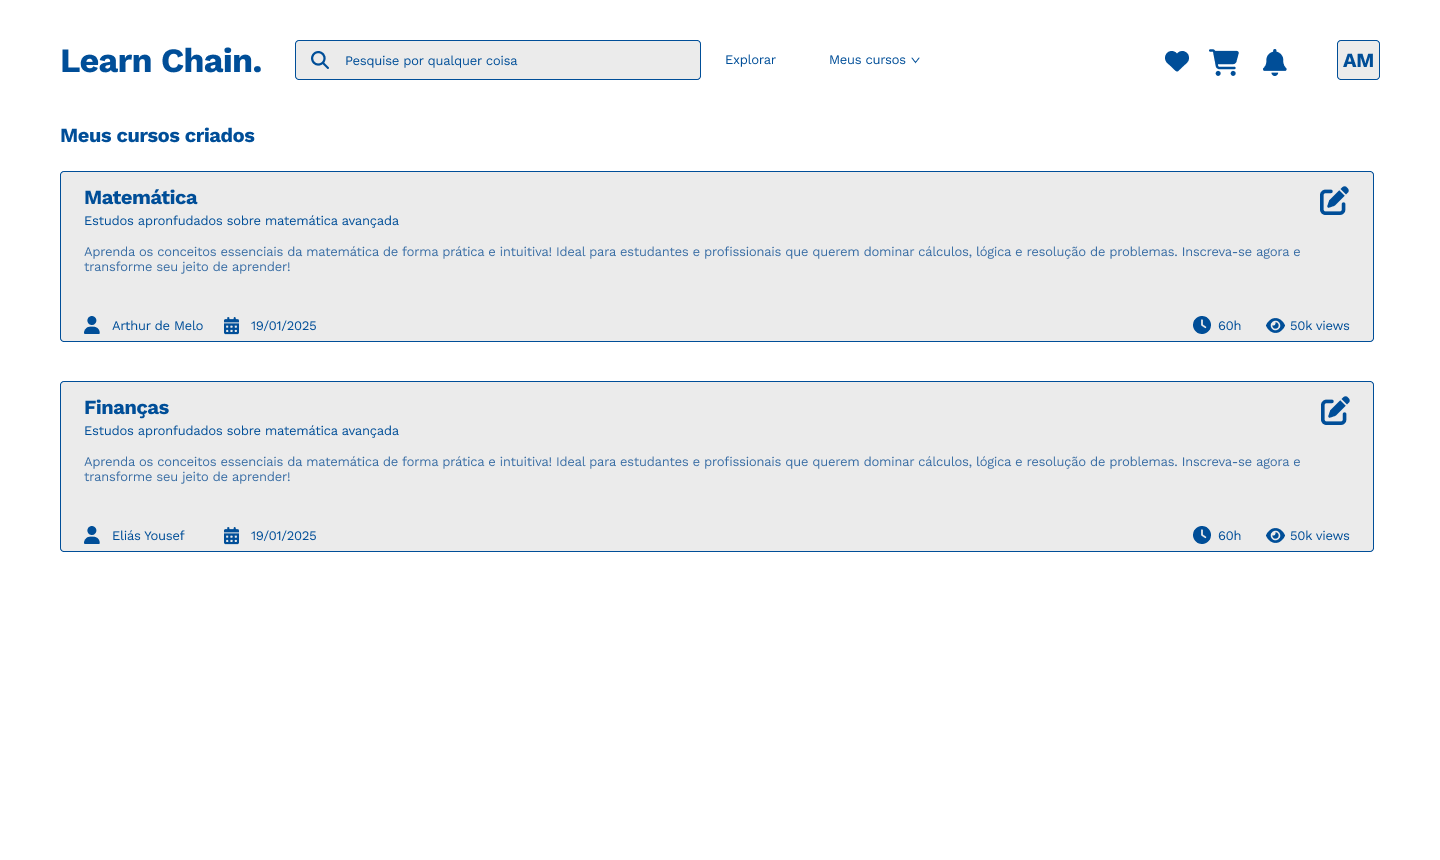
\includegraphics[width=0.8\textwidth]{figuras/meus_cursos.png}
        \begin{center}
            {\footnotesize Fonte: Autores}
        \end{center}
        \label{fig:meus_cursos}
    \end{figure}

    \begin{figure}[h]
        \centering
        \caption{Edição/Criação de cursos}
        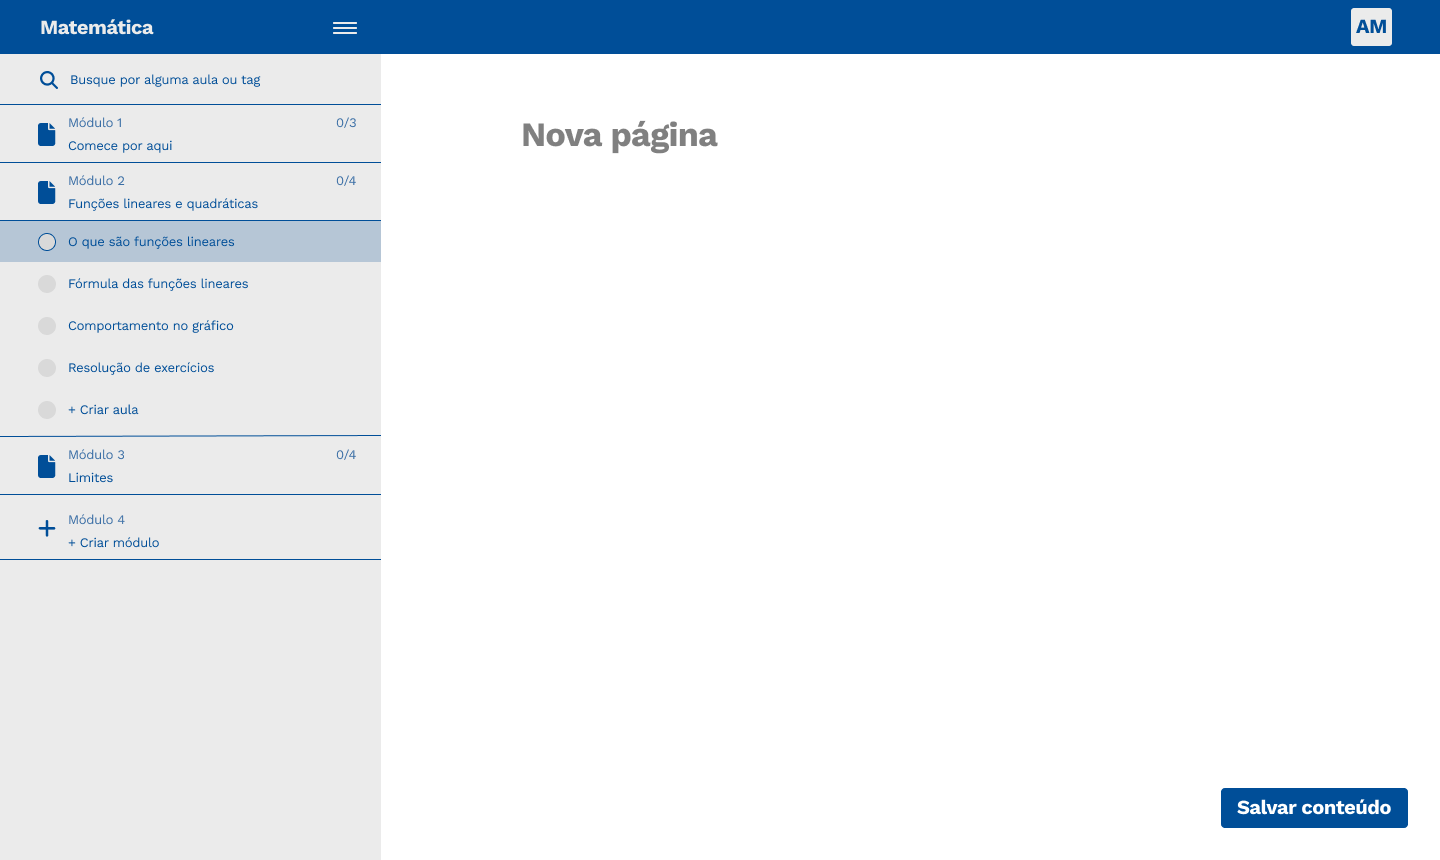
\includegraphics[width=0.8\textwidth]{figuras/Criando_curso.png}
        \begin{center}
            {\footnotesize Fonte: Autores}
        \end{center}
        \label{fig:Criando_curso}
    \end{figure}

    \begin{figure}[h]
        \centering
        \caption{Diagrama Lógico de Dados}
        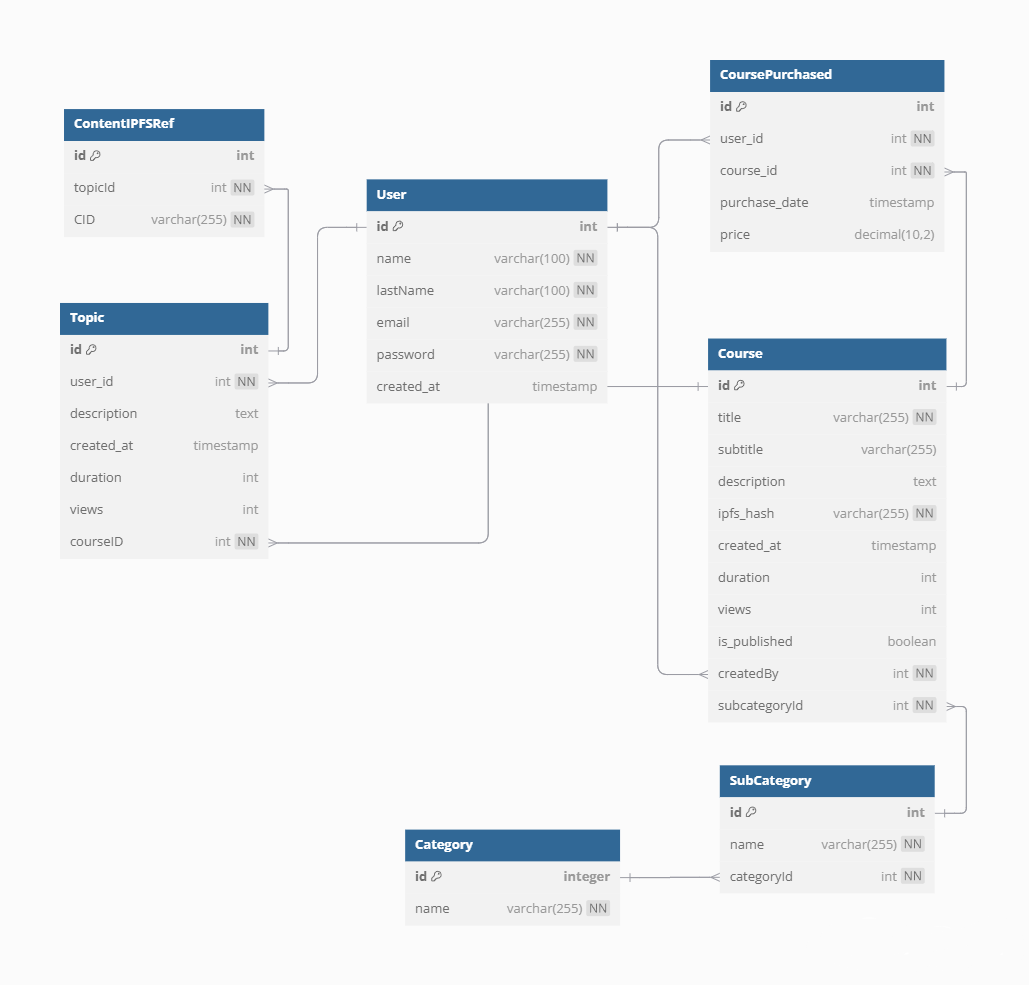
\includegraphics[width=0.8\textwidth]{figuras/ddl.png}
        \begin{center}
            {\footnotesize Fonte: Autores}
        \end{center}
        \label{fig:dld}
    \end{figure}

\chapter{Brainstorming}
\label{cap:brainstorming}
    \begin{figure}[h]
        \centering
        \caption{Brainstorming desenvolvido pessoalmente}
        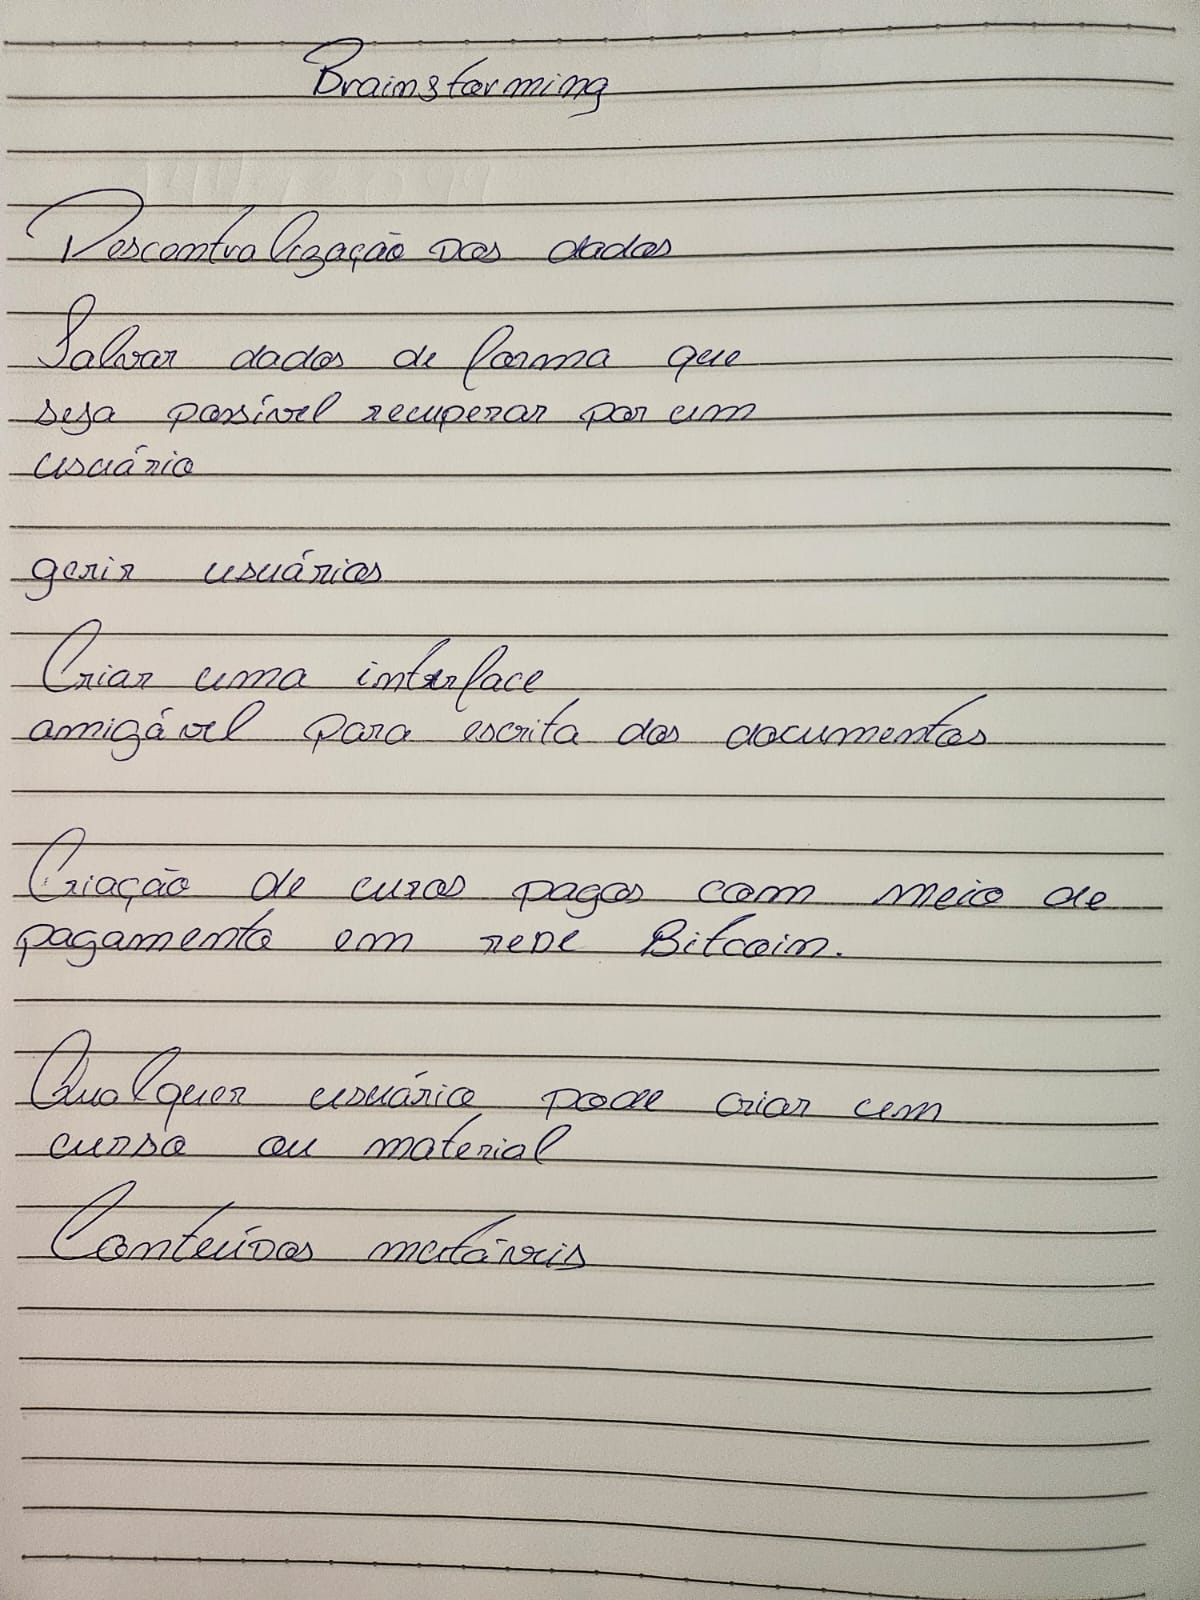
\includegraphics[width=0.8\textwidth]{figuras/brainstorming-presencial.png}
        \begin{center}
            {\footnotesize Fonte: Autores}
        \end{center}
        \label{fig:brainstorming-pessoal}
    \end{figure}

    \begin{figure}[h]
        \centering
        \caption{Brainstorming desenvolvido remotamente}
        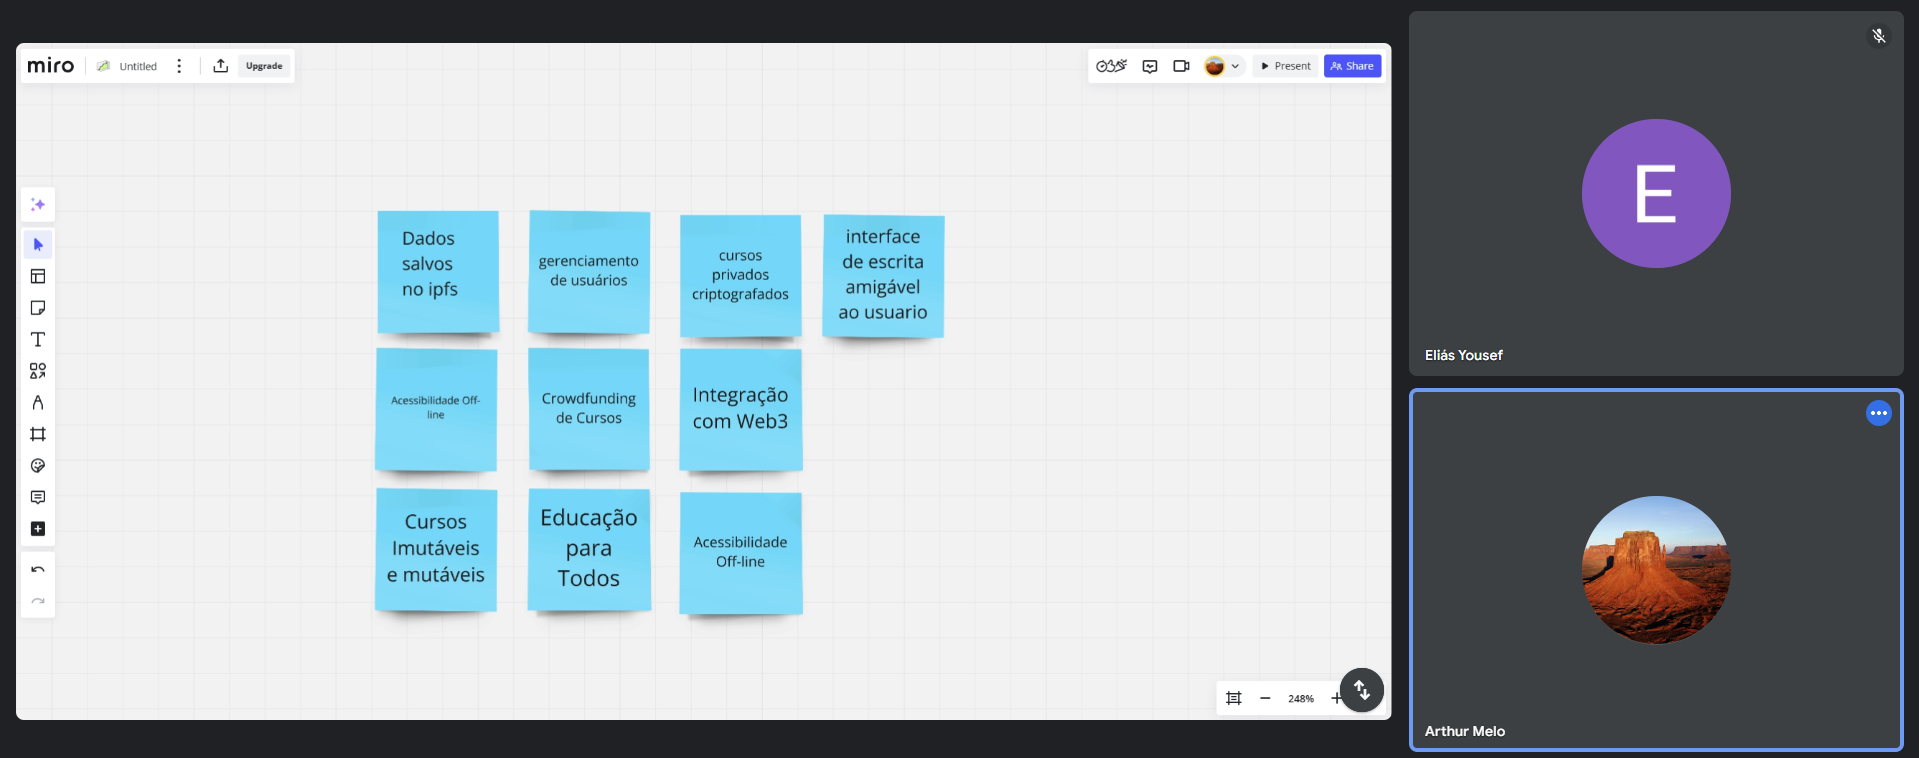
\includegraphics[width=0.8\textwidth]{figuras/BrainsStorming online.png}
        \begin{center}
            {\footnotesize Fonte: Autores}
        \end{center}
        \label{fig:brainstorming-remoto}
    \end{figure}

\end{apendicesenv}
